\documentclass[12pt,a4paper]{article}
\usepackage[left=2.5cm,right=2.5cm,top=2.5cm,bottom=2.5cm]{geometry}
\usepackage[utf8]{inputenc}
\usepackage{amssymb, amsmath, amsthm}
\usepackage{hyperref}
\usepackage{algorithmic, algorithm}
\usepackage{graphics, graphicx}
\graphicspath{ {./8.4/} }
\DeclareMathOperator*{\argmax}{argmax}
\pagestyle{empty}
\hypersetup{
  colorlinks   = true, %Colours links instead of ugly boxes
  urlcolor     = blue, %Colour for external hyperlinks
}

\begin{document}
\textbf{Chapter 8 solutions  \hfill Hanna Gábor}

\begin{enumerate}
  \item
    \textit{The nonplanning method looks particularly poor in Figure 8.3 because it is
    a one-step method; a method using multi-step bootstrapping would do better. Do you
    think one of the multi-step bootstrapping methods from Chapter 7 could do as well as
    the Dyna method? Explain why or why not.}

    I think it can come close. An $n$-step bootstrpping algorithm with big enough $n$ (or a
    Monte Carlo method) would update at the end of the first episode all the action-values we
    encountered during the episode.
    I expect the policy based on these updated action-values to be quite good.

  \item
    \textit{Why did the Dyna agent with exploration bonus, Dyna-Q+, perform
    better in the first phase as well as in the second phase of the blocking and shortcut
    experiments?}

    At first, both algorithms might find an okay policy that is suboptimal. Due
    to the exploration, Dyna-Q+ will realize it sooner that it's a suboptimal policy.

  \item
    \textit{Careful inspection of Figure 8.5 reveals that the difference between Dyna-Q+
    and Dyna-Q narrowed slightly over the first part of the experiment. What is the reason
    for this?}

    After finding the optimal path, Dyna-Q always uses that path, whereas Dyna-Q+
    does some exploration from time to time.

  \item
    \textit{Programming. The exploration bonus described above actually changes
    the estimated values of states and actions. Is this necessary? Suppose the bonus
    $\kappa \sqrt{\tau}$ was used not in updates, but solely in action selection.
    That is, suppose the action selected was always that for which $Q(S_t, a) +
    \kappa \sqrt{\tau (S_t, a)}$ was maximal. Carry out a gridworld experiment
    that tests and illustrates the strengths and weaknesses of this alternate approach.}

    My expectation is that in some cases it's worse to use the bonus only in the
    action selection. Suppose that we need a series of exploratory steps to find
    the shortcut. If we update the actual values, then once the exploration bonus
    is big enough, we will soon find the shortcut. If we only use the bonus for action
    selection, it might happen that we take one exploratory step but before reaching the
    shortcut, we get back to the old path. If this happens, we will need to wait until
    the first exploratory step accumulates a huge bonus again to go down on that
    path again.

    I couldn't reproduce the cumulative reward of $400$ shown in the book, my
    implementation of Dyna-Q+ only reached $350$ and I couldn't figure out why.
    Anyway, here is the result.

    \begin{center}
    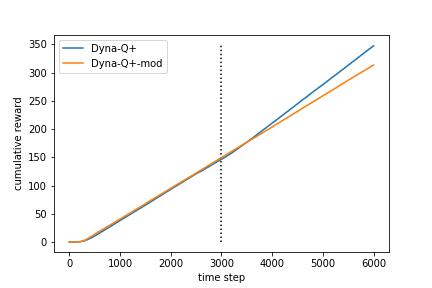
\includegraphics[scale=0.7]{dyna}
    \end{center}

  \item
    \textit{How might the tabular Dyna-Q algorithm shown on page 164 be modified
    to handle stochastic environments? How might this modification perform poorly on
    changing environments such as considered in this section? How could the algorithm be
    modified to handle stochastic environments and changing environments?}

    Instead of assigning single reward-state pairs to state-action pairs in the model,
    we could store all the reward-state pairs that we've seen after taking the
    respective action. We would sample from these stored items during the planning
    phase. To handle changes in the environment, we could modify this to sample
    only from the $k$ latest reward-state pairs.


\end{enumerate}
\end{document}
